\documentclass[oneside]{article}
\bibliographystyle{plain}
\usepackage{amssymb,amsmath,graphicx}
\begin{document}
\title{Preserving Antebellum Print Culture}
\author{Jason Peak}
%\maketitle


\def\projectname{Poe's Magazine World}
\def\apc{Antebellum Print Culture}
\def\bwj{\emph{The Broadway Journal}}
\def\slm{\emph{Southern Literary Messenger}}
\def\bgm{\emph{Burton's Gentleman's Magazine}}
\def\gm{\emph{Graham's Magazine}}
\def\maglist{\bgm, \bwj, \gm, and the \slm}

%TODO
\def\needcite{[citation]}
\def\needswork{[needs much work for inclusion]}

%begin content
%\begin{abstract}
%\projectname, a digital humanities project centered around the literary culture of the 1840s in America, seeks to accumulate and present digital artifacts that re-contextualize this period in history for future readers, students and researchers. The project team is composed of a cross-disciplinary mix of scholars and students committed to establishing a research archive for the equally diverse audience of scholarly researchers, students and the general public. At its broadest, the scope of the project includes all American Antebellum authors and would take shape as part of a consortium of linked archives. As a first step, however, the project will focus on Poe's involvement with four periodicals, the \bwj{}, \slm{}, \bgm{} and \gm{}.
%\end{abstract}

%\section{Project Description}
%Understanding the project domain, background, goals and roadmap are essential to asserting the way forward. The domain of the project is hierarchical, and at its most general, it includes everything that can be defined as \emph{\apc}. Recognizing that small steps begin a great journey, the APC group have wisely decided to begin with a narrower scope, specifically, the writings of Edgar Allen Poe. As the first step, they have chosen to focus on his work as editor of periodicals. That effort is the subject of this discussion.

\subsection{Domain}
Poe is famous for his tales and poetry, indeed, every grade school child has been thrilled by \emph{The Raven}, for instance. It is probably less well-known that in his capacity as an editor of several periodicals, he took the opportunity to offer commentary on the events and cultural themes that mark the American Antebellum period. The \projectname project will draw attention to this aspect of the author and his perspective by creating a digital collection of four of the periodicals in which he played a key editorial role: \maglist. 

\subsection{Background}
The \apc project has been underway for a few years, and in that time, there has been much discussion and converging general agreement over exactly what the content of the repository should be and how to best present it. In the last year, the project has focused its efforts around presenting a proof-of-concept prototype exploring three Poe tales. From a technical perspective, this has been achieved through adoption and customization of the Omeka web publishing platform. More will be said about Omeka later on, but for now, suffice it to say that the Omeka prototyping effort has exposed important requirements of the project, specifically, needs for:
\begin{enumerate}
  \item{a user-friendly management interface to the repository}
  \item{flexible content presentation options}
  \item{fine-grained metadata schemes}
  \item{semantic relationships between entities, especially at the sub-document level}
\end{enumerate}

\subsection{Goals}
\subsection{Core Goals and Requirements}
For the editions of the magazines that Poe edited, the page count is about 4,000. The primary project goal is the establishment of a digital repository containing the text and scanned image of each of these pages. In addition to making each page image available,the text should be fully searchable. Providing access to page images and text search tools implies an access-controlled, web-based interface. Maintaing the integrity of complex, mixed-media, multipage document records requires sturdy archival frameworks and flexible metadata standards. 


\subsection{Stretch}
With core foundation blocks laid, the team will build up enhanced access services, including annotation, semantic search, and the infrastructure to expose the repository as linked open data. 
\begin{description}
  \item[Annotation] consists of moderated user annotations to the elements of the repository. These annotations may become part of the archival record.   
  \item[Search] entails semantic markup. The team will identify or develop an appropriate ontology with which to describe semantic relationships amongst repository elements at the sub-document level. Initial candidates for such markup include people, places, corporate bodies captured with EAC-CPF. 
  \item[Linked Open Data] Client webservices will be developed  to allow others to reuse the archive as a dataset for their own purposes. 
\end{description}



%\section{Project Domain}
%
\begin{description}
  \item[Scan]{Each of the 4,000 pages contained in the corpus in scope will be scanned to high resolution TIFF}
  \item[Extract]{OCR and minimal human processing will result in level 2 TEI\cite{tei_sig_on_libraries_best_2011} markup for each page}
  \item[Preserve]{These artifacts must be preserved in a trusted system}
\end{description}

As a result of these three tasks, the initial phase will establish a trusted digital repository (TDR) suitable as a research resource. Facilities for research will include, at a minimum, document retrieval and full-text search. With these basic foundation blocks firmly laid, other services can be built that further enhance the value of this resource for research including scholarly annotation, use of RDF for making semantic inferences, and a range of client web services that expose the archive to other repositories and applications.


\subsection{Core Goals and Requirements}
For the editions of the magazines that Poe edited, the page count is about 4,000. The primary project goal is the establishment of a digital repository containing the text and scanned image of each of these pages. In addition to making each page image available,the text should be fully searchable. Providing access to page images and text search tools implies an access-controlled, web-based interface. Maintaing the integrity of complex, mixed-media, multipage document records requires sturdy archival frameworks and flexible metadata standards. 


\subsection{Stretch}
With core foundation blocks laid, the team will build up enhanced access services, including annotation, semantic search, and the infrastructure to expose the repository as linked open data. 
\begin{description}
  \item[Annotation] consists of moderated user annotations to the elements of the repository. These annotations may become part of the archival record.   
  \item[Search] entails semantic markup. The team will identify or develop an appropriate ontology with which to describe semantic relationships amongst repository elements at the sub-document level. Initial candidates for such markup include people, places, corporate bodies captured with EAC-CPF. 
  \item[Linked Open Data] Client webservices will be developed  to allow others to reuse the archive as a dataset for their own purposes. 
\end{description}

%\section{Requirements}
%sh: compile.sh: No such file or directory
\begin{description}
  \item[Archival Preservation] The APC project requires trustworthy archival preservation of its primary artifacts, derivative scholarship and interactions.
    \section{TDR}
    \begin{quote}A sustainable, trustworthy, well-supported, and well-managed digital repository needs hardware, software, policies, processes, services, and people to assure long-term retention and, perhaps, access to its content and metadata.\cite{dow_elizabeth_2009} \end{quote}
The term Trusted Digital Repository implies that there can be digital repositories that are not trusted. Dow uses the term \emph{Trustworthy} Digital Repository to describe a repository that is defined by an \emph{overall commitment to the stewardship of digital materials}\cite{dow_elizabeth_2009}. Further, she says that 
  \item[Exposure] Artifacts and their metadata must be exposed to client applications including search engines, browsers, and visualization applications
  \item[Granular markup] Text documents will be encoded in the TEI at the various levels enumerated in \cite{tei_sig_on_libraries_best_2011} 
\end{description}

\section{New Tools}
At the base, there  must be a robust and trusted repository in which born-digital artifacts are deposited. The time and expense required to capture this corpus deserves no less, and we imagine that generations of future scholars and students will benefit from our efforts, provided that the materials are well-preserved in accordance with the best practices currently known to the archives community. 

\subsection{TDR}
\begin{quote}A sustainable, trustworthy, well-supported, and well-managed digital repository needs hardware, software, policies, processes, services, and people to assure long-term retention and, perhaps, access to its content and metadata.\cite{dow_elizabeth_2009} \end{quote}
The term Trusted Digital Repository implies that there can be digital repositories that are not trusted. Dow uses the term \emph{Trustworthy} Digital Repository to describe a repository that is defined by an \emph{overall commitment to the stewardship of digital materials}\cite{dow_elizabeth_2009}. Further, she says that 

\section{Current Infrastructure}
Currently, the project uses the popular Omeka publishing platform as repository, content ingest and administration interface, and dissemination portal. The application relies on a relational database to maintain application state and configuration, to control user access, for persistent records and metadata storage, and for RDF-like inter-record relationship data. 

Besides offering a one-stop solution to the needs of a small repository, Omeka is freely available and open source from top to bottom. It is written in PHP and based on the industry standard Zend PHP framework. It can be fitted to a number of databases, including PostgreSQL and MySQL, which are also free and open source. Rounding out the Omeka architecture is the apache webserver running on linux. Using open source software allows the team great flexibility in customizing the software, and independence in resolving technical issues. As the project goals outgrow the capabilities of Omeka, finding a similarly open replacement will be in keeping with archival best practices \needcite




\section{Formats and Standards}
\subsection{File Formats}

\begin{description}
  \item[Image]{TIFF image format will be required}
  \item[Text][all non0-image files will be XML]
\end{description}

\subsection{XML Formats}
\begin{description}
  \item[TEI]{}
  \item[METS]{}
  \item[MODS]{}
  \item[DC]{}
\end{description}

\subsection{Standards}
\begin{description}
  \item[DRAMBORA]{}
\end{description}



\section{Workflow}
Workflow is loosely defined here. Inevitably, refinements will be made as issues are discovered and resolved. The acquisition process, from capture to ingest, can be imagined as a pipeline starting from the physical original and ending with an archival Submission Information Package (SIP). Stages in this pipeline include: 
\begin{enumerate}
  \item{Scan}
  \item{OCR}
  \item{OCR correction}
  \item{TEI markup}
  \item{packaging}
\end{enumerate}
%This chain of functions can be represented as $SIP ::= TEI(text(scan(page)))$
While each stage will require human intervention and oversight, the OCR correction stage is expected to incur the most significant outlay of human resources. 
\subsection{Scan}
We intend to use facilities in the Hill Memorial Library for the bulk of the scans. This equipment is designed to scan a full page spread, two facing pages, at a time, but each page is saved as a discrete file. Scanning will be applied to each page in each issue of each periodical in the project scope.



The scanning process will operate at the page level and will require manual operation. It will take as input physical original peridical pages and return as output a simgle high resolution TIFF image per page and text extracted through OCR. The products of this process are the basis of the archive.
\begin{description}
  \item[periodical]{physical original magazine}
  \item[page]{leaf of a periodical}
  \item[scan]{digitization of leaf to TIFF}
  \item[TIFF]{image of leaf}
  \item[OCR]{process by which text is extracted from TIFF}
  \item[raw text]{output of OCR}
  \item[OCR correction]{manual process by which machine interpretation errors are corrected by humans}
  \item[TEI-1]{baseline format of text for archival storage}
  \item[SIP]{METS-encoded record of a single periodical issue containing TIFF + TEI of each leaf contained in the original}
\end{description}



\section{Migration}
To date, a great deal of content has been located in collections, scanned and stored in the Omeka repository. Because Omeka is open source, developing a migration path for existing records will require careful execution, but little difficulty or uncertainty. Further, there is no technical or economic reason that this will need to be done in haste, as may be the case in a hosted environment where each megabyte incurs a certain cost per hosted minute. 
\subsection{Transition}
Once an alternative platform is chosen, selected and thoroughly tested, the Omeka site can be put into a read-only state such that no further modifications to its records database can occur. With the database frozen, a full database backup, using mysqldump, will create a fixed-point snapshot of the database state, a restoration point.
\subsection{Translation}
Using knowledge gained in the course of developing custom Omeka plugins, data translation scripts will marshall complete records from the Omeka database tables and render each as a SIP ingestible by the new system. With all of its records safely ingested in the new system, the old system will remain in read-only state as a reference for as long as the team deems useful (probably a year).

\section{Information Structure}
\subsection{METS Records}
METS is a structural description and container format that can wrap other formats including TEI, RDF, MODS, EAD, etc. It enjoys widespread use and the endorsement of leading archival institutions, including the Library of Congress. As a structural description format, it is an ideal choice for storing records of multipage documents \needcite. Fedora uses METS.


\section{Questions}
\begin{enumerate}
  \item{What examples of RDF + Fedora exist?}
  \item{describe the mapping from DC -> METS; is this automated in Fedora}
  \item{}
\end{enumerate}

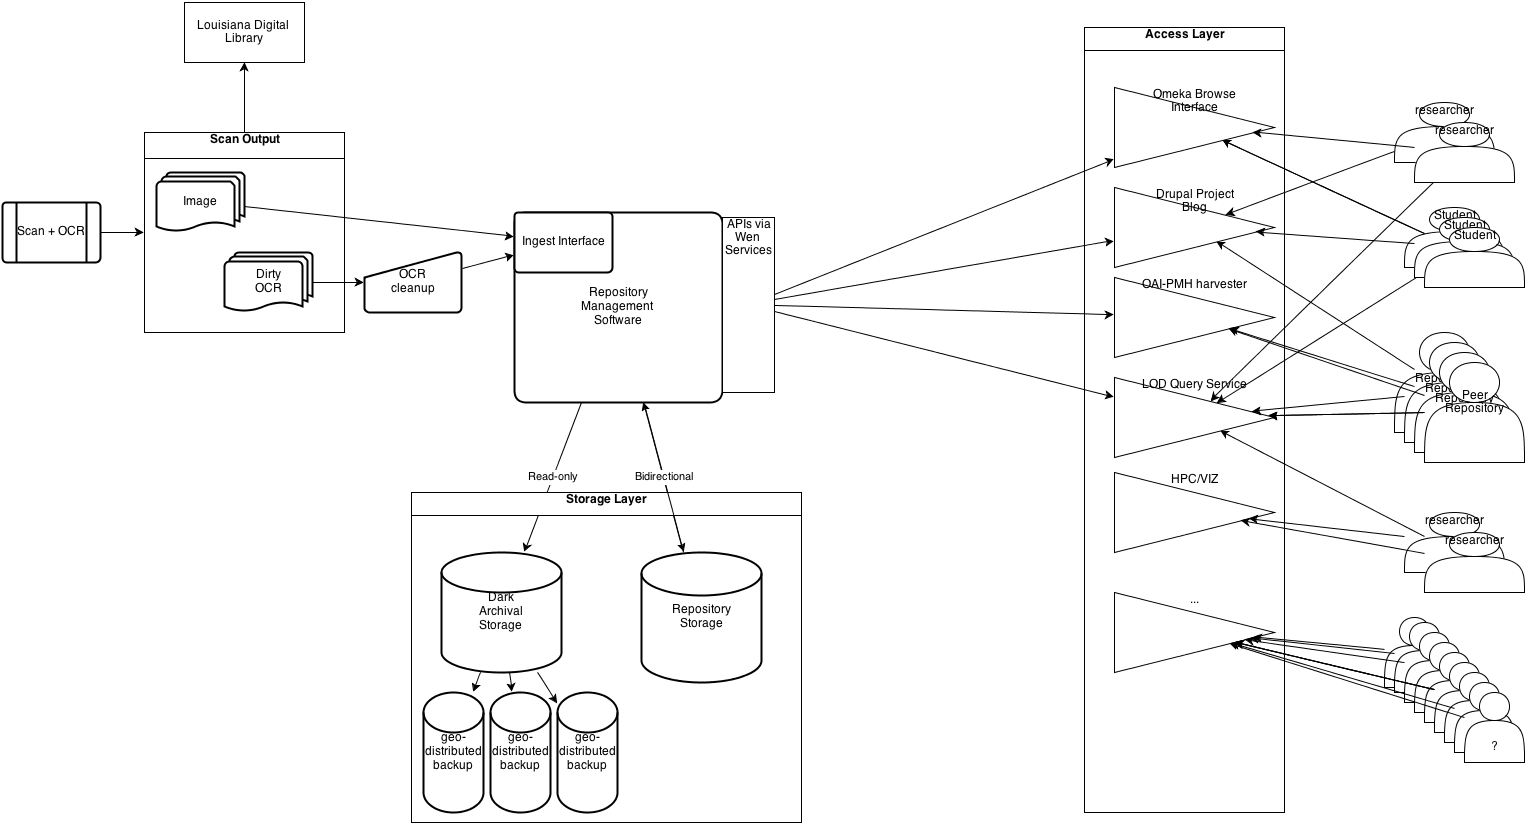
\includegraphics[width=\textwidth]{apc-01.png}

\subsection{Semantic web}
Further, in an increasingly interconnected and socially interlinked world, the digital archive assumes a certain burden to provide its content to patrons (researchers, students, the public) in increasingly compelling ways. One of the most promising technologies for achieving this end is embodied in the concept of the Semantic Web \needcite[TBL]. The semantic web represents an inductive step beyond the character of the web we've grown to know in the last several decades. In this new web, hyperlinks are not merely a means by which to refer to some other, arbitrary, web resource, rather, the reference itself is imbued with an additional dimension that describes the nature of the relationship between the thing and what it points to. \needcite[Barthes?] Employing such technology in an archives setting improves discoverability by expanding the role of the archive from simple document retrieval to something much richer.

\bibliography{bib}

\end{document}
